\section{Marco teórico}
\subsection{Sitios de CQA}
\begin{frame}
	\frametitle{Sitios de CQA}
	\begin{tcolorbox}[colback=blue!5,colframe=blue!40!black,title=Sitios de Community Question Answering]
		Los sitios de \textit{Community Question Answering} CQA, son un tipo especial de sitios web de \textit{Question Answering} (QA), los cuales permiten a los usuarios registrados responder a preguntas formuladas por otras personas.
	\end{tcolorbox}
\end{frame}

\subsection{Sistemas de recomendación}
\begin{frame}
	\frametitle{Sistemas de Recomendación}
	\begin{tcolorbox}[colback=blue!5,colframe=blue!40!black,title=Sistemas de Recomendación]
		Un RS es un conjunto de herramientas de software que sugiere ítems a un usuario, quien posiblemente utilizará algunos de ellos.
	\end{tcolorbox}

	\bigskip

	\textbf{Funciones de un Sistema de Recomendación}
	\begin{itemize} [<*>]
		\item Aumentar el ratio de conversión en un sitio o aplicación.
		\item Aumentar satisfación y fidelidad del usuario.
	\end{itemize}
\end{frame}

\subsection{Big Data y Arquitecturas}
\begin{frame}[allowframebreaks]
	\frametitle{Big Data}
	\begin{tcolorbox}[colback=blue!5,colframe=blue!40!black,title=Big Data]
		``Conjuntos de datos cuyo tamaño está más allá de la habilidad de las herramientas software de base de datos para capturar, almacenar, gestionar y analizar los datos'' (Manyika et al., 2011).

		\bigskip

		``Big Data son activos de información caracterizados por su alto volumen, velocidad y variedad que demandan formas innovadoras y rentables de procesamiento de información para mejorar la compresión y la toma de decisiones'' (consultora Gartner).
	\end{tcolorbox}
\end{frame}

\subsection{Medidas de distancia de texto}
\begin{frame}
	\frametitle{Similaridad}
	Las medidas de similaridad son de interés para poder cuantificar la relación entre objetos.
	\bigskip
	\begin{itemize}
		\item Se utilizan dos tipos de medidas de similaridad en este trabajo:
		\begin{enumerate}[<*>]
			\item Basadas en espacios vectoriales.
			\item Basadas en taxonomías.
		\end{enumerate}

		\bigskip
		\item
		La función de similaridad es definida satisfaciendo las condiciones:
		\begin{enumerate}[<*>]
			\item Simetría,
			\[S(x_i,x_j)=S(x_j,x_i);\]

			\item Positividad,
			\[0 \leq S(x_i,x_j) \leq 1, \quad \forall x_i,x_j.\]
		\end{enumerate}
		\medskip
		Es posible transformar una medida de similaridad \(S(x_i,x_j)\) en una de distancia \(D(xi,xj)\) que cumpla \(0 \leq D(x_i,x_j) \leq 1\), en el intervalo \([0,1]\). Aplicando \(D(x_i,x_j) = 1 - S(x_i,x_j)\).
	\end{itemize}
\end{frame}

\begin{frame}
	\frametitle{Modelo de espacio vectorial}
	En el modelo de \textit{espacio vectorial}, un texto es representado como un vector de términos. Si las palabras son elegidas como términos, entonces cada palabra del vocabulario sería una \textit{dimensión} independiente en el espacio vectorial (Singhal et al., 2001).

	\bigskip

	Típicamente, el ángulo entre los dos vectores es usado como medida de divergencia entre los mismos, y el coseno del ángulo es usado como similaridad numérica.
\end{frame}

\begin{frame}[allowframebreaks]
	\frametitle{Similaridad del coseno}
	La distancia del coseno se puede derivar de la fórmula del \textit{producto escalar}:
	\[\vec{D}_i.\vec{D}_j = \left \| \vec{D}_i \right \|.\left \| \vec{D}_j \right \|.cos(\theta),\]
	siendo \(\left \|\overrightarrow{D_i}\right \|\) y \(\left \|\overrightarrow{D_j}\right \|\) los módulos de los vectores \(\overrightarrow{D_i}\) y \(\overrightarrow{D_j}\) respectivamente, y $\theta$ el ángulo formado entre ellos.

	\bigskip

	La similaridad entre dos vectores puede medirse como:
	\[cos(\theta) = \frac{\vec{D}_i.\vec{D}_j}{\left \| \vec{D}_i \right \|.\left \| \vec{D}_j \right \|},\]
	donde \(d_i\) y \(d_j\) son los componentes de los vectores \(\overrightarrow{D_i}\) y \(\overrightarrow{D_j}\) respectivamente.
\end{frame}

\begin{frame}[allowframebreaks]
	\frametitle{Similaridad en taxonomías}
		\begin{figure}
		\centering
		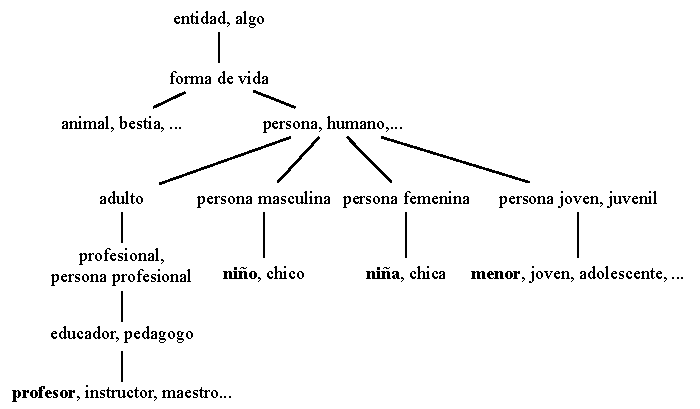
\includegraphics[width=0.7\linewidth]{../7_marco_teorico/imagenes/taxonomia_semantica}
		\label{fig:taxonomiasemantica}
	\end{figure}

	\begin{footnotesize}
		La similaridad entre palabras se define como \(S(w_1,w_2)=f(l,h),\)
		donde \(l\) es el camino más corto entre \(w_1\) y \(w_2\), y \(h\) es la profundidad del subsumer de las mismas.
	\end{footnotesize}

	\framebreak

	Se define \(p(t)\) como la \textbf{probabilidad} de un concepto \(t\), formalizando:
	\[p(t)=\frac{freq(t)}{N},\]

	\bigskip

	Se define el \textbf{contenido de información} \(I(t) = 0\) como:
	\[I(t)=-\log p(t).\]

	Entonces la \textbf{similaridad} entre dos términos \((i, j)\) se define como:
	\[S_R = I(ms(t_i,t_j)),\; (Resnik,\,1995)\]

	\[S_L(t_i, t_j)=\frac{2S_R(t_i,t_j)}{I(t_i)+I(t_j)}.\; (Lin\,et\,al.,\,1998)\]
\end{frame}

\begin{frame}
	\frametitle{Medidas de Similaridad}
	\textbf{Medidas de similaridad utilizadas}
	\bigskip
	\begin{itemize}[<*>]
		\item Term Frequency (TF)
		\item Term Frequency - Inverse Docuement Frequency (TF-IDF).
		\item Word2Vec
		\item FastText
		\item Semantic Distance
	\end{itemize}
\end{frame}

\begin{frame}
	\frametitle{Term Frequency (TF)}
	Caracteristicas de Term Frequency:
	\bigskip
	\begin{itemize}[<*>]
		\item También conocido en la literatura como \textit{Bag of words} (bolsa de palabras).
		\item El orden exacto de los términos es ignorado, pero se basa en el número de ocurrencias de cada uno de ellos en un documento.
		\item Cada documento corresponde a un vector y cada término a una dimensión.
		\item Se mide el grado de similaridad de dos documentos utilizando el coseno del ángulo entre dos vectores.
	\end{itemize}

	\bigskip
	\centering
	\textit{“Mary is quicker than John”} y \textit{“John is quicker than Mary”} \\
	\medskip
	\begin{scriptsize}
		(``Mary es más rápida que John'' y ``John es más rápido que Mary'')
	\end{scriptsize}
\end{frame}

\begin{frame}
	\frametitle{Term Frequency Inverse Document Frequency (TF-IDF)}
	Caracteristicas de TF-IDF:
	\bigskip
	\begin{itemize}[<*>]
		\item Se define \textit{document frequency} \(df_t\) como el número de documentos en una colección que contienen el término \(t\).
		\item \textit{Inverse document frequency}, o IDF, es un indicador basado en la cantidad de documentos que contienen (o son indexados por) un término en cuestión.
		\item Intuición: si un término de búsqueda se encuentra en muchos documentos, no es un buen discriminador, y se le debe asignar menor peso que a un término que se encuentra en pocos documentos.
	\end{itemize}

	\centering
	\[tfidf(t_i, d_j) = tf(t_i, d_j) \cdot idf(t_j)\]
\end{frame}

\begin{frame}
	\frametitle{Word2Vec}
	Caracteristicas de Word2Vec:
	\bigskip
	\begin{itemize}[<*>]
		\item Modelos basados en redes neuronales con una capa oculta para computar representaciones de palabras como vectores continuos en grandes conjuntos de datos.
		\item Dos modelos: Skip-gram y Continuous Bag of Words.
		\item Las entradas y salidas de la red neuronal son palabras representadas como \textit{one-hot} vector.
		\item Los pesos de la capa oculta se van ajustando utilizando un clasificador de regresión Softmax.
		\item Estos pesos resultantes dan como resultado a la representación vectorial de palabras utilizadas para el cálculo de similaridad de este trabajo.
	\end{itemize}
\end{frame}

\begin{frame}
	Caracteristicas de FastText:
	\bigskip
	\frametitle{FastText}
	\begin{itemize}[<*>]
		\item Libreria open-source desarrollada por Facebook.
		\item Basado en Skip-gram pero utilizando un modelo sub-palabra.
		\item Cada palabra es representada como una bolsa de \textit{n-gramas}.
		\item Mayor precisión en diferentes medidas de rendimiento.
	\end{itemize}
\end{frame}

\begin{frame}[allowframebreaks]
	\frametitle{Semantic Distance}
	Caracteristicas de Semantic Distance:
	\bigskip
	\begin{itemize}[<*>]
		\item La distancia semántica usada en este trabajo está basada en \textit{redes semánticas} y \textit{estadísticas de corpus} (Li et al., 2006).
		\item Enfocado en textos de distancia corta.
		\item Tiene en cuenta la \textit{información semántica} y la \textit{información del orden} de las palabras implicadas en las frases involucradas.
	\end{itemize}

	\begin{figure}
		\centering
		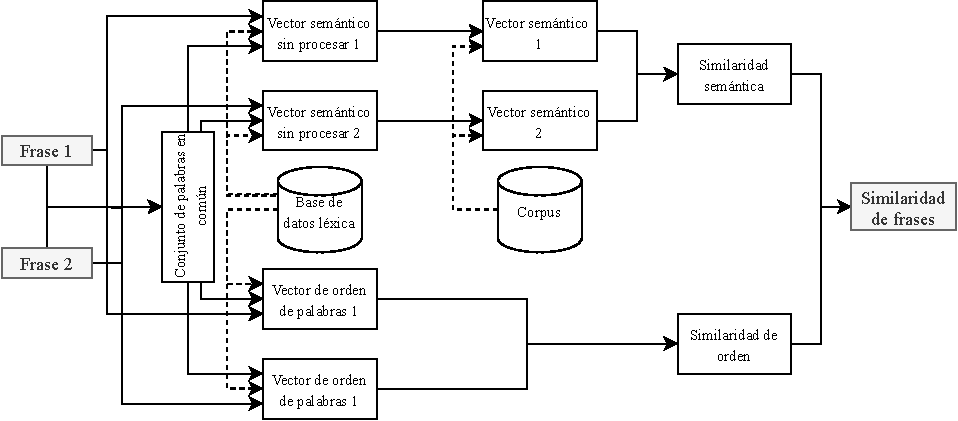
\includegraphics[width=0.7\linewidth]{../7_marco_teorico/imagenes/similaridad_sematinca_metodo}
		\label{fig:similaridadsematincametodo}
	\end{figure}

	\framebreak

	\textbf{Similaridad semántica entre frases} \\
	\bigskip
		Un conjunto de palabras comunes \(T\) es formado por la unión de las dos frases \(T_1\) y \(T_2\) en comparación. Luego, un vector semántico léxico \(\check{s}\) es derivado de este conjunto. Por cada una de las palabras \(w_i\) en \(T\) \textit{(ejemplo para \(T_1\))}:
	\begin{itemize}[<*>]
		\item \textbf{Caso 1}. Si \(w_i\) aparece en la \(T_1\), \(s_i\) es 1.
		\item \textbf{Caso 2}. Si \(w_i\) no está contenida en \(T_1\), se calcula una similaridad semántica entre \(w_1\) y cada palabra en \(T_1\) utilizando el método de similaridad entre palabras.
	\end{itemize}

	\bigskip
	Luego el vector semántico de cada frase es:
	\[s_i = \check{s} \cdot I(w_i) \cdot I(\widetilde{w}_i),\]

	Entonces, la similaridad semántica entre dos frases es definida como el coeficiente del coseno entre los dos vectores.

	\framebreak

	\textbf{Similaridad de orden entre frases} \\
	\bigskip
	Consideremos dos frases \(T_1\) y \(T_2\), por ejemplo:
	\begin{itemize}[<*>]
		\item \textbf{T1}: A quick brown dog jumps over the lazy fox.
		\item \textbf{T2}. A quick brown fox jumps over the lazy dog.
	\end{itemize}

	\bigskip
	Se define un conjunto \(T\) con la union de las palabras en \(T_1\) y \(T_2\) y luego se definen los vectores de orden:
	\[r_1 = \left \{\;1\;2\;3\;4\;5\;6\;7\;8\;9\;\right \},\]
	\[r_2 = \left \{\;1\;2\;3\;9\;5\;6\;7\;8\;4\;\right \}.\]

	Se propone entonces una medida de similaridad de orden entre frases de la siguiente manera:
	\[S_r = 1 - \frac{\left \| r_1 - r_2 \right \|}{\left \| r_1 + r_2 \right \|}.\]

	\framebreak

	\textbf{Similaridad total entre frases:} \\
	\bigskip

	\[S(T_1, T_2)=\delta S_s + (1 - \delta)S_r,\]
	\[S(T_1, T_2)=\delta \frac{s_1.s_2}{\left \| s_1 \right \|\left \| s_2 \right \|} + (1 - \delta)\frac{\left \|r_1-r_2 \right \|}{\left \| r_1+r_2 \right \|},\]

	\bigskip
	donde \(0 \leq \delta \leq 1\) decide la contribución relativa de cada una de las medidas de similaridad.
\end{frame}

\subsection{Ensamble de Clustering}
\begin{frame}
	\frametitle{Ensamble de Clustering}
	\begin{tcolorbox}[colback=blue!5,colframe=blue!40!black,title=Ensamble de Clustering]
		El \textit{Ensamble de Clustering} es un método para extraer clusters consistentes dadas particiones variadas de entrada.
	\end{tcolorbox}

 	\bigskip

	\begin{itemize}
		\item Combina resultados de distintos algoritmos de Clustering con clusters de distintas formas.
		\item Aprovecha la variabilidad agregada para encontrar una estructura \textit{inter-patrón}.
		\item Identificación de clusters subyacentes con formas, tamaños y densidades arbitrarias.
	\end{itemize}
\end{frame}

\begin{frame}
	\frametitle{Combinación de Evidencias}
	Tomado las co-ocurrencia de pares de patrones en el mismo cluster, las \(N\) particiones de datos para \(n\) patrones, son mapeadas en una \textit{matriz de co-asociación} \(n \times n\):
	\medskip
	\[C(i,j)=\frac{n_{ij}}{N},\]
	\medskip
	donde \(n_{ij}\) es el número de veces que el par de patrones \((i,j)\) es asignado al mismo cluster entre las \(N\) particiones de datos.
\end{frame}
